\documentclass[tikz]{standalone}
\usepackage{amsmath,amssymb}
\usepackage{pgfplots,multicol}

\pgfplotsset{compat=1.13}
\usepgfplotslibrary{fillbetween}

\begin{document}


 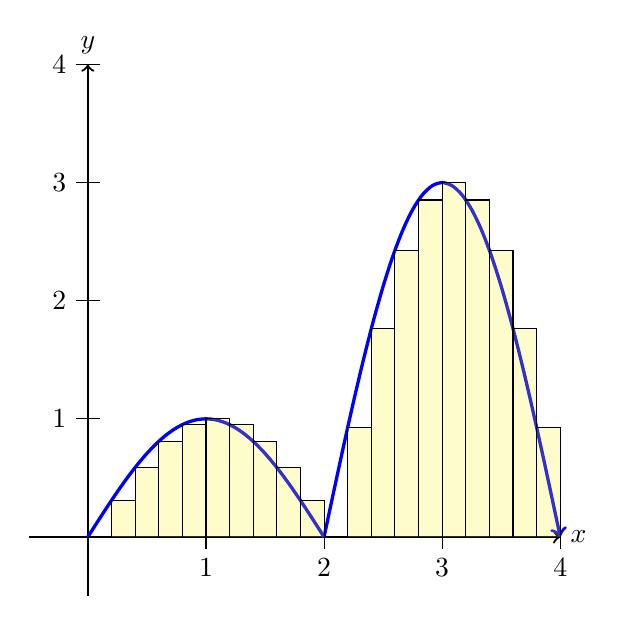
\begin{tikzpicture}[scale=1.5,	declare function={ f(\x) =abs(sin(\x*90)); g(\x) =3*abs(sin(\x*90)); 
                 }]
        \draw[->,thick] (-0.5,0) -- (4,0) node[right] {$x$};
    \draw[->,thick] (0,-0.5) -- (0,4) node[above] {$y$};
	\foreach \x in {1,2,3,4} \draw (\x,0.1) -- (\x, -0.1) node[below] {\x};
	\foreach \y in {1,2,3,4} \draw (0.1,\y) -- (-0.1, \y) node[left] {\y};
	\draw[-,smooth,domain=0:2,very thick,blue] plot(\x,{f(\x)});
	\draw[->,smooth,domain=2:4,very thick,blue] plot(\x,{g(\x)});
	

\foreach \t in {0,0.2,0.4,0.6,0.8,1,1.2,1.4,1.6,1.8} \draw[fill=yellow, fill opacity=0.2] (\t,0) -- (\t,{f(\t)}) -- ({\t+0.2}, {f(\t)}) -- ({\t+0.2},0);

\foreach \t in {2,2.2,2.4,2.6,2.8,3,3.2,3.4,3.6,3.8} \draw[fill=yellow, fill opacity=0.2] (\t,0) -- (\t,{g(\t)}) -- ({\t+0.2}, {g(\t)}) -- ({\t+0.2},0);
	

\end{tikzpicture}

	
\end{document}
